\section{Training the Generative Model}
\label{sec:training_generative_models}
In the last two sections, we showed how to construct a generative model with a vector field $u_t^\theta$ given by a neural network, and we derived a formula for the training target $\uref_t$. In this section, we will describe how to train the neural network $u_t^\theta$ to approximate the training target $\uref_t$. First, we restrict ourselves to ODEs again, in doing so recovering \themebf{flow matching}. Second, we explain how to extend the approach to SDEs via \themebf{score matching}. Finally, we consider the special case of Gaussian probability paths, in doing so recovering \themebf{denoising diffusion models}. With these tools, we will at last have an end-to-end procedure to train and sample from a generative model with ODEs and SDEs.

\subsection{Flow Matching}

As before, let us consider a flow model given by
\begin{align}
\label{eq:ode_model}
 X_0&\sim\pinit,\quad \dd X_t = u_t^\theta(X_t)\,\dd t. &&\blacktriangleright\,\,\text{flow model}
\end{align}
As we learned, we want the neural network $u_t^\theta$ to equal the marginal vector field $\uref_t$. In other words, we would like to find parameters $\theta$ so that $u_t^\theta\approx \uref_t$. In the following, we denote by $\text{Unif}=\text{Unif}_{[0,1]}$ the uniform distribution on the interval $[0,1]$, and by $\mathbb{E}$ the expected value of a random variable. An intuitive way of obtaining $u_t^\theta\approx \uref_t$ is to use a mean-squared error, i.e. to use the \themebf{flow matching loss} defined as
\label{subsec:training_algorithm}
\begin{align}
    \label{eq:marginal_loss_function}
\Lmarg(\theta)&=\mathbb{E}_{t\sim\text{Unif},x\sim p_t}[\|u_t^\theta(x) - \uref_t(x)\|^2]\\&\overset{(i)}{=} \mathbb{E}_{t\sim\text{Unif},z\sim \pdata, x\sim p_t(\cdot|z)}[\|u_t^\theta(x) - \uref_t(x)\|^2],
\end{align}
where $p_t(x)=\int p_t(x|z)\pdata(z) \dd z$ is the marginal probability path and in $(i)$ we used the sampling procedure given by \cref{eq:marginal_prob_path}. Intuitively, this loss says: First, draw a random time $t \in [0,1]$. Second, draw a random point $z$ from our data set, sample from $p_t(\cdot|z)$ (e.g., by adding some noise), and compute $u_t^\theta(x)$. Finally, compute the mean-squared error between the output of our neural network and the marginal vector field $\uref_t(x)$. Unfortunately, we are \textit{not} done here. While we do know the formula for $\uref_t$ by \cref{thm:marginalization_trick}
\begin{align}
\label{eq:marginal_vector_field_stated_again}
    \uref_t(x) = \int \uref_t(x|z)\frac{ p_t(x|z)\pdata(z)}{p_t(x)}\dd z,
\end{align}
we cannot compute it efficiently because the above integral is intractable. Instead, we will exploit the fact that the \themebf{conditional} velocity field $\uref_t(x|z)$ is tractable. % We could try to approximate the above integral by screening over the whole dataset. However, even for a dataset of 1 million images (which is very small in modern days), we would need to loop over 1 million images every time we evaluate $\uref_t(x)$ - an extremely computationally expensive approach. However, it turns out that we can solve this. 
To do so, let us define the \themebf{conditional flow matching loss} 
\begin{align}
\label{eq:cfm}
\Lcond(\theta) =     \mathbb{E}_{t\sim \Unif, z\sim \pdata, x\sim p_t(\cdot|\dap)}[\|u_t^\theta(x) - \uref_t(x|\dap)\|^2].
\end{align}
Note the difference to     \cref{eq:marginal_loss_function}: we use the conditional vector field $\uref_t(x|z)$ instead of the marginal vector $\uref_t(x)$. As we have an analytical formula for $\uref_t(x|z)$, we can minimize the above loss easily. But wait, what sense does it make to regress against the conditional vector field if it's the marginal vector field we care about? As it turns out, by \themeit{explicitly} regressing against the tractable, conditional vector field, we are \themeit{implicitly} regressing against the intractable, marginal vector field. The next result makes this intuition precise.

\begin{theorem}
\label{thm:fm_loss} 
The marginal flow matching loss equals the conditional flow matching loss up to a constant. That is,
\begin{align*}
\Lmarg(\theta) = \Lcond(\theta) + C,
\end{align*}
where $C$ is independent of $\theta$. Therefore, their gradients coincide:
\begin{align*}
\nabla_\theta \Lmarg(\theta) = \nabla_\theta \Lcond(\theta).
\end{align*}
Hence, minimizing $\Lcond(\theta)$ with e.g., stochastic gradient descent (SGD) is equivalent to minimizing $\Lmarg(\theta)$ with in the same fashion. In particular, for the minimizer $\theta^*$ of $\Lcond(\theta)$, it will hold that $u_t^{\theta^*}=\uref_t$ (assuming an infintely expressive parameterization). 
\end{theorem}
\begin{proof}
The proof works by expanding the mean-squared error into three components and removing constants:
\begin{align*}
    \Lmarg(\theta)&\overset{(i)}{=}\mathbb{E}_{t\sim\text{Unif},x\sim p_t}[\|u_t^\theta(x) - \uref_t(x)\|^2]\\
    &\overset{(ii)}{=}\mathbb{E}_{t\sim\text{Unif},x\sim p_t}[\|u_t^\theta(x)\|^2 - 2u_t^\theta(x)^T\uref_t(x) + \|\uref_t(x)\|^2]\\
    &\overset{(iii)}{=}\mathbb{E}_{t\sim\text{Unif},x\sim p_t}\left[\|u_t^\theta(x)\|^2\right] - 2\mathbb{E}_{t\sim\text{Unif},x\sim p_t}[u_t^\theta(x)^T\uref_t(x)] + \underbrace{\mathbb{E}_{t\sim\text{Unif}_{[0,1]}, x\sim p_t}[\|\uref_t(x)\|^2]}_{=:C_1}\\
    &\overset{(iv)}{=}\mathbb{E}_{t\sim\text{Unif},z\sim\pdata, x\sim p_t(\cdot|z)}[\|u_t^\theta(x)\|^2] - 2\mathbb{E}_{t\sim\text{Unif},x\sim p_t}[u_t^\theta(x)^T\uref_t(x)] + C_1
\end{align*}
where $(i)$ holds by definition, in $(ii)$ we used the formula $\|a-b\|^2=\|a\|^2-2a^Tb+\|b\|^2$, in $(iii)$ we define a constant $C_1$ and in $(iv)$ we used the sampling procedure of $p_t$ given by \cref{eq:marginal_prob_path}. Let us reexpress the second summand:
\begin{align*}
\mathbb{E}_{t\sim\text{Unif},x\sim p_t}[u_t^\theta(x)^T\uref_t(x)]&\overset{(i)}{=}\int\limits_{0}^{1}\int p_t(x)u_t^\theta(x)^T\uref_t(x)\,\dd x\, \dd t\\
&\overset{(ii)}{=}\int\limits_{0}^{1}\int p_t(x)u_t^\theta(x)^T\left[\int \uref_t(x|z)\frac{ p_t(x|z)\pdata(z)}{p_t(x)}\dd z\right]\dd x\, \dd t\\
&\overset{(iii)}{=}\int\limits_{0}^{1}\int\int u_t^\theta(x)^T\uref_t(x|z) p_t(x|z)\pdata(z)\,\dd z\,\dd x\, \dd t\\
&\overset{(iv)}{=}\mathbb{E}_{t\sim\text{Unif},z\sim \pdata, x\sim p_t(\cdot|z)}[u_t^\theta(x)^T\uref_t(x|z)]
\end{align*}
where in $(i)$ we expressed the expected value as an integral, in $(ii)$ we use \cref{eq:marginal_vector_field_stated_again}, in $(iii)$ we use the fact that integrals are linear, in $(iv)$ we express the integral as an expected value. Note that this was really the crucial step of the proof: The beginning of the equality used the marginal vector field $\uref_t(x)$, while the end uses the conditional vector field $\uref_t(x|z)$. We plug is into the equation for $\Lmarg$ to get:
\begin{align*}
\Lmarg(\theta)&\overset{(i)}{=}\mathbb{E}_{t\sim\text{Unif},z\sim \pdata, x\sim p_t(\cdot|z)}[\|u_t^\theta(x)\|^2]-2\mathbb{E}_{t\sim\text{Unif},z\sim \pdata, x\sim p_t(\cdot|z)}[u_t^\theta(x)^T\uref_t(x|z)] +C_1\\
&\overset{(ii)}{=}\mathbb{E}_{t\sim\text{Unif},z\sim \pdata, x\sim p_t(\cdot|z)}[\|u_t^\theta(x)\|^2-2u_t^\theta(x)^T\uref_t(x|z)+\|\uref_t(x|z)\|^2-\|\uref_t(x|z)\|^2] +C_1\\
&\overset{(iii)}{=}\mathbb{E}_{t\sim\text{Unif},z\sim \pdata, x\sim p_t(\cdot|z)}[\|u_t^\theta(x)-\uref_t(x|z)\|^2]+\underbrace{\mathbb{E}_{t\sim\text{Unif},z\sim \pdata, x\sim p_t(\cdot|z)}[-\|\uref_t(x|z)\|^2]}_{C_2} +C_1\\
&\overset{(iv)}{=}\Lcond(\theta) + \underbrace{C_2+C_1}_{=:C}
\end{align*}
where in $(i)$ we plugged in the derived equation, in $(ii)$ we added and subtracted the same value,  in $(iii)$ we used the formula $\|a-b\|^2=\|a\|^2-2a^Tb+\|b\|^2$ again, and in $(iv)$ we defined a constant in $\theta$. This finishes the proof.
\end{proof}
Once $u_t^{\theta}$ has been trained, we may simulate the flow model
\begin{align}
\label{eq:sde_extension_restated}
    \dd X_t = u_t^\theta(X_t)\, \dd t,\quad\quad X_0\sim\pinit
\end{align}
via e.g., \cref{alg:sampling_flow_model} to obtain samples $X_1\sim \pdata$. This whole pipeline is called \themebf{flow matching} in the literature \citep{lipman2022flow, liu2022flow, albergo2023stochastic, lipman2024flow}. The training procedure is summarized in \cref{alg:training_fm_score_matching_gaussian_paths} and visualized in \cref{fig:fm_illustration_checkerboard}. Let us now instantiate the conditional flow matching loss for the choice of Gaussian probability paths:
\begin{examplebox}[Flow Matching for Gaussian Conditional Probability Paths]
Let us return to the example of Gaussian probability paths $p_t(\cdot|z)=\mathcal{N}(\alpha_t z; \beta_t^2 I_d)$, where we may sample from the conditional path via
\begin{align}
\label{eq:sampling_procedure_gaussian_path_restated_for_fm}
    \epsilon\sim\mathcal{N}(0,I_d)\quad 
    \Rightarrow\quad x_t = \alpha_t z + \beta_t \epsilon \sim \mathcal{N}(\alpha_tz,\beta_t^2I_d)=p_t(\cdot|z).
\end{align}
As we derived in \cref{eq:conditional_gaussian_vf}, the conditional vector field $\uref_t(x|z)$ is given by
\begin{align}
\label{e:marginal_vf_cond_score}
    \uref_t(x|z) =& \left(\dot{\alpha}_t-\frac{\dot{\beta}_t}{\beta_t}\alpha_t\right)z+\frac{\dot{\beta}_t}{\beta_t}x,
\end{align}
where $\dot{\alpha}_t=\partial_t\alpha_t$ and $\dot{\beta}_t=\partial_t\beta_t$ are the respective time derivatives. Plugging in this formula, the conditional flow matching loss reads
\begin{align*}
\Lcond(\theta) &= \mathbb{E}_{t\sim \text{Unif},z\sim \pdata, x\sim \mathcal{N}(\alpha_tz,\beta_t^2I_d)}[\lVert u_t^\theta(x)-\left(\dot{\alpha}_t-\frac{\dot{\beta}_t}{\beta_t}\alpha_t\right)z-\frac{\dot{\beta}_t}{\beta_t}x\rVert^2]\\&\overset{(i)}{=}\mathbb{E}_{t\sim\Unif,z\sim \pdata, \epsilon\sim \mathcal{N}(0,I_d)}[\|u_t^\theta(\alpha_tz+\beta_t\epsilon)-(\dot{\alpha}_tz+\dot{\beta}_t\epsilon)\|^2]
\end{align*}
where in $(i)$ we plugged in \cref{eq:sampling_procedure_gaussian_path_restated_for_fm} and replaced $x$ by $\alpha_tz+\beta_t\epsilon$. Note the simplicity of $\Lcond$ : We sample a data point $z$, sample some noise $\epsilon$ and then we take a mean squared error. Let us make this even more concrete for the special case of $\alpha_t=t$, and $\beta_t=1-t$. The corresponding probability $p_t(x|z)=\mathcal{N}(tz,(1-t)^2)$ is sometimes referred to as the (Gaussian) \themebf{CondOT probability path}. Then we have $\dot{\alpha}_t=1,\dot{\beta}_t=-1$, so that
\begin{align*}
        \mathcal{L}_{\text{cfm}}(\theta)=&\mathbb{E}_{t\sim\Unif,z\sim \pdata, \epsilon\sim \mathcal{N}(0,I_d)}[\|u_t^\theta(tz+(1-t)\epsilon)-(z-\epsilon)\|^2]
\end{align*}
Many famous state-of-the-art models have been trained using this simple yet effective procedure, e.g. \themeit{Stable Diffusion 3}, Meta's \themeit{Movie Gen Video}, and probably many more proprietary models. In \cref{fig:fm_illustration_checkerboard}, we visualize it in a simple example and in \cref{alg:training_fm_score_matching_gaussian_paths} we summarize the training procedure.
\end{examplebox}
\begin{algorithm}[h]
\caption{Flow Matching Training Procedure (here for Gaussian CondOT path $p_t(x|z)=\mathcal{N}(tz,(1-t)^2)$)}
\label{alg:training_fm_score_matching_gaussian_paths}
\begin{algorithmic}[1]
\REQUIRE A dataset of samples $z\sim \pdata$, neural network $u_t^\theta$
\FOR{each mini-batch of data}
    \STATE Sample a data example $\dap$ from the dataset.
    \STATE Sample a random time $t \sim \text{Unif}_{[0,1]}$.
    \STATE Sample noise $\epsilon\sim\mathcal{N}(0,I_d)$
    \STATE Set $x=t z + (1-t) \epsilon$\hfill (\text{General case: }$x\sim p_t(\cdot|z)$)
    %\IF{Flow matching}
    \STATE Compute loss
    \begin{align*}
        \mathcal{L}(\theta) =& \|u_t^\theta(x)-(z-\epsilon)\|^2 \quad &(\text{General case: }=\|u_t^\theta(x)-\uref_t(x|z)\|^2)
    \end{align*}
    %\ENDIF
    % \IF{Score matching}
    % \STATE
    % \begin{align*}
    %     \mathcal{L}(\theta) =& \|s_t^\theta(x_t)+\frac{\epsilon}{\beta_t}\|^2 \quad &(\text{General case: }=\|s_t^\theta(x_t)+\nabla\log p_t(x_t|z)\|^2)
    % \end{align*}
    % \ENDIF
    \STATE Update the model parameters $\theta$ via gradient descent on $\mathcal{L}(\theta)$.
\ENDFOR
\end{algorithmic}
\end{algorithm}
\begin{figure}[!t]
    \centering
    \begin{tabular}{ccc}
         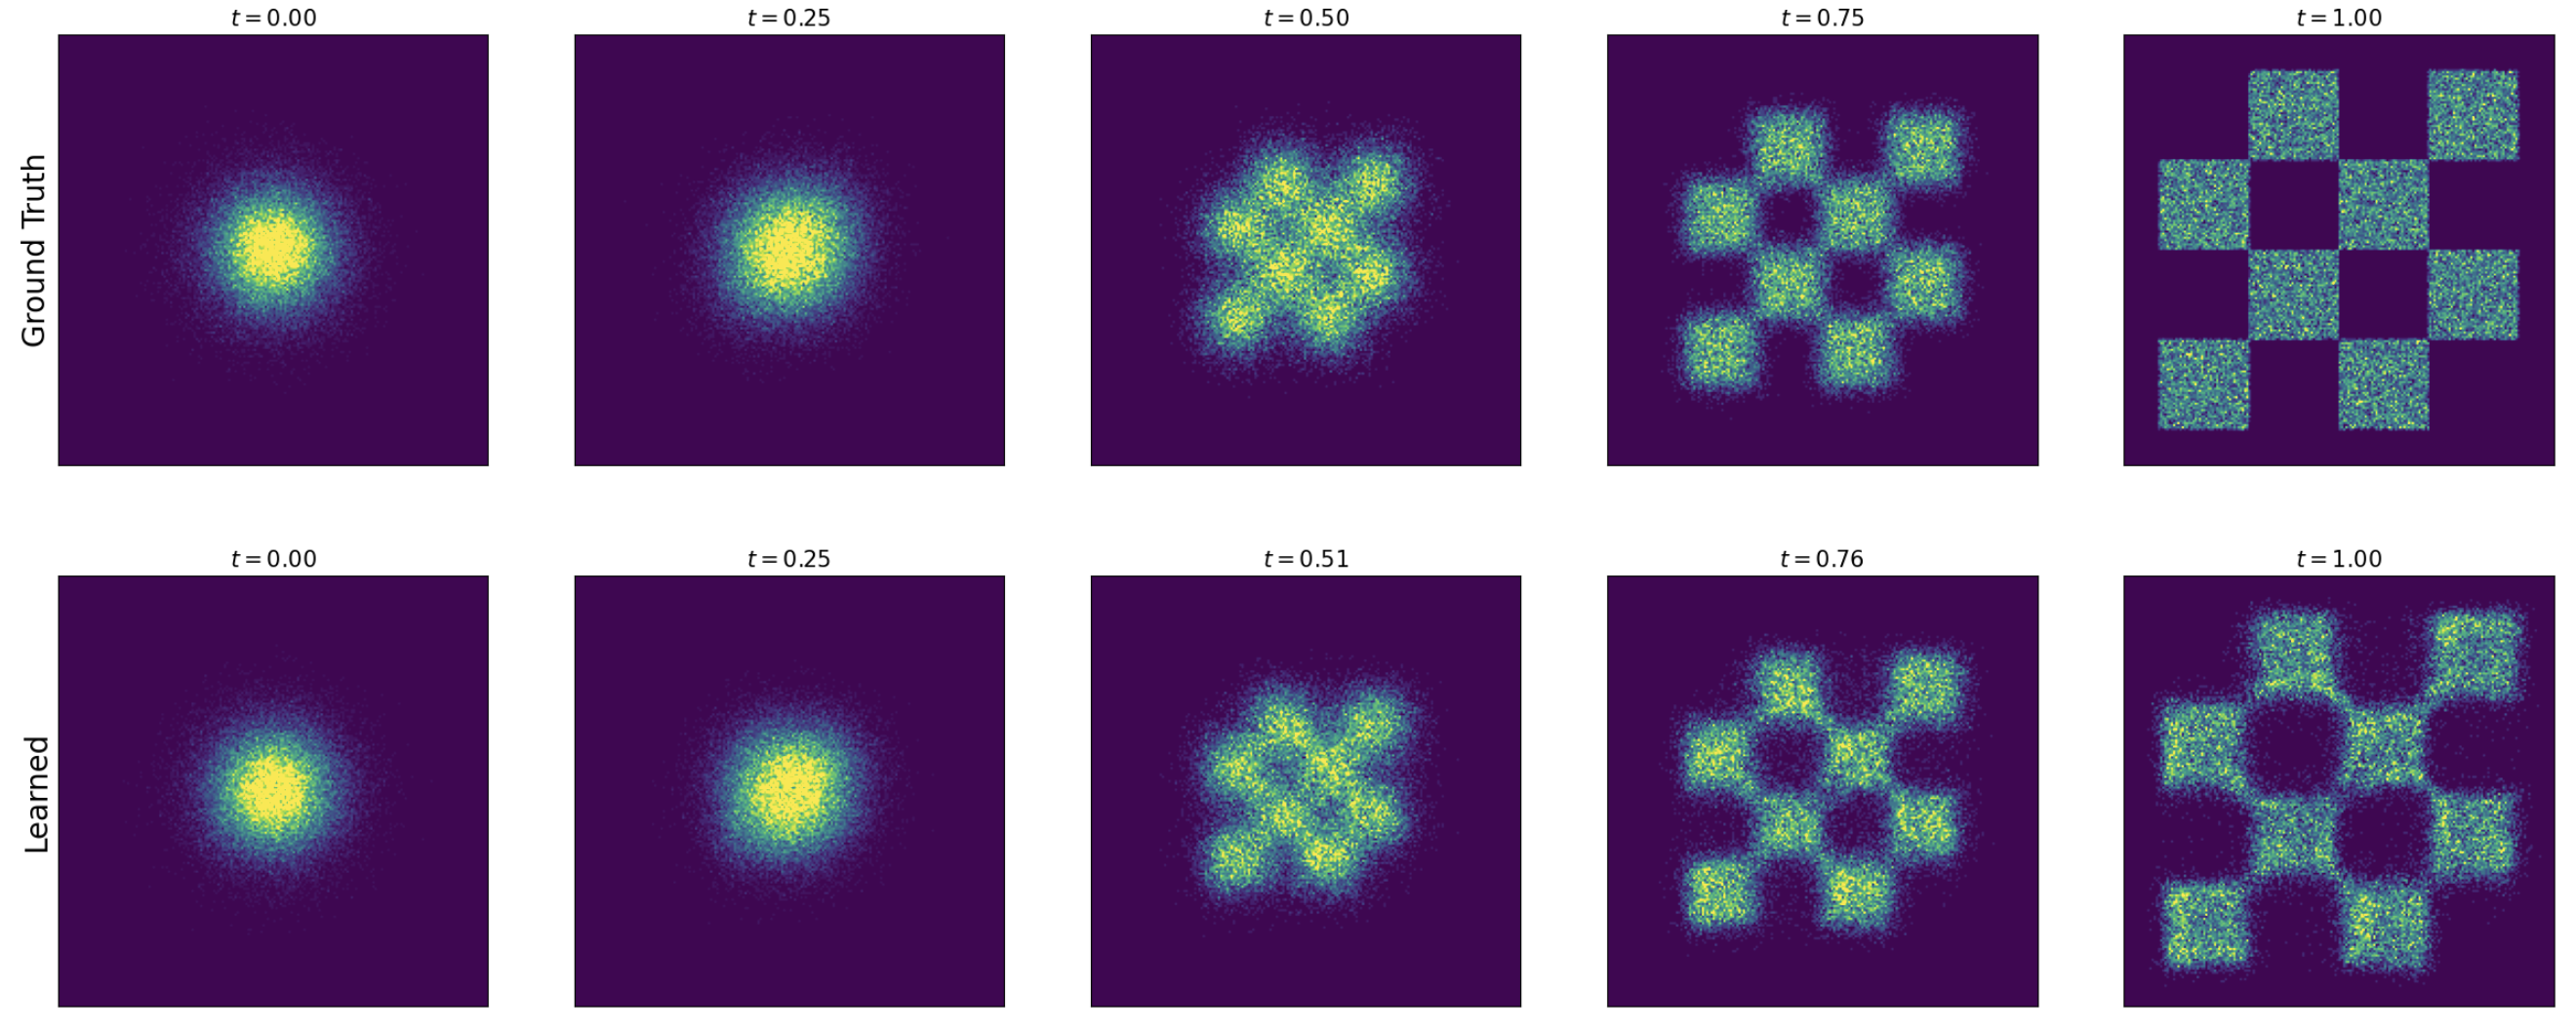
\includegraphics[width=\textwidth]{figures/conditional_marginal_path.png} &
         % \includegraphics[width=0.22\textwidth]{assets/flow_velocity/flow_v_5.png} &
         % 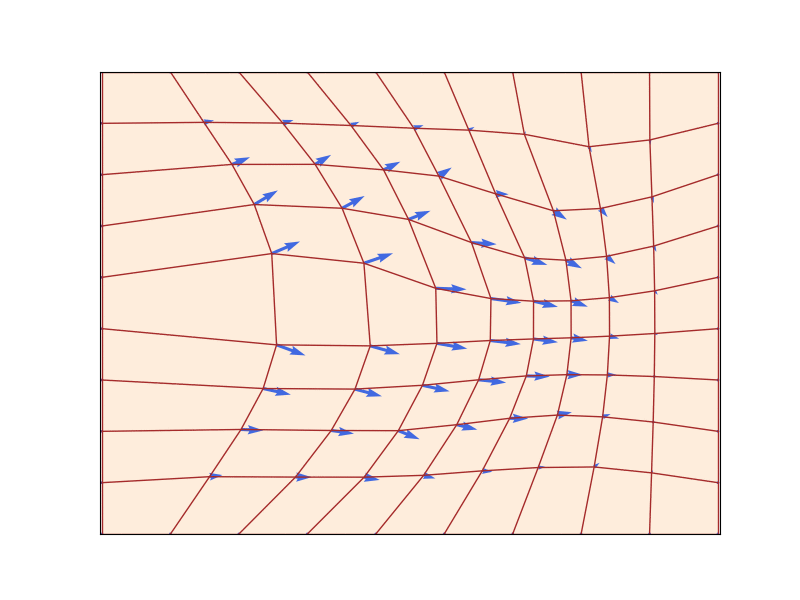
\includegraphics[width=0.3\textwidth]{fm_guide_assets/flow_10.png} &
         % % \includegraphics[width=0.22\textwidth]{assets/flow_velocity/flow_v_14.png} &
         % 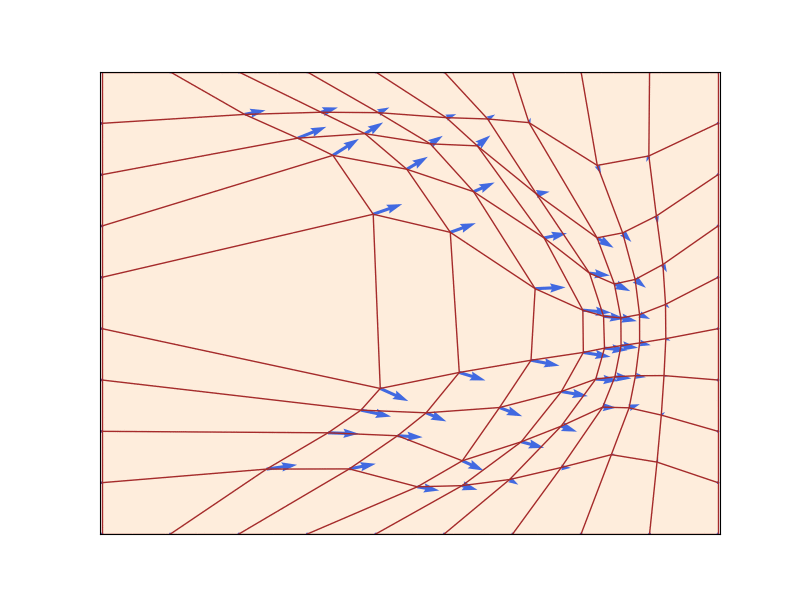
\includegraphics[width=0.3\textwidth]{fm_guide_assets/flow_16.png} 
    \end{tabular}
    \caption{\label{fig:fm_illustration_checkerboard}Illustration of \cref{thm:fm_loss} with a Gaussian CondOT probability path: simulating an ODE from a trained flow matching model. The data distribution is the chess board pattern (top right). Top row: Histogram from ground truth marginal probability path $p_t(x)$. Bottom row: Histogram of samples from flow matching model. As one can see, the top row and bottom row match after training (up to training error). The model was trained using \cref{alg:training_fm_score_matching_gaussian_paths}.}
\end{figure}

% When I first saw \cref{thm:fm_loss}, I found it a big magical: Without seeing $\uref_t(x)$ explicitly ever, we can approximate it implicitly with a neural network. Therefore, \cref{thm:fm_loss} gives us a powerful of training our ODE generative model by minimizing $\Lcond(\theta)$. All we have to do is minimize a simple mean squared error. This is scalable to very large datasets in high dimensions and can be implemented in a few lines of code. When tracking the training, you should keep in mind that \textbf{the absolute value of the loss is meaningless} (you will never achieve zero loss because $C<0$). This makes it sometimes a little tricky to realize when the training is converged.
\subsection{Score Matching}

Let us extend the algorithm we just found from ODEs to SDEs. Remember we can extend the target ODE to an SDE with the same marginal distribution given by
\begin{align}
\label{eq:sde_extension_restated}
    \dd X_t &=\left[\uref_t(X_t)+\frac{\sigma_t^2}{2}\nabla\log p_t(X_t)\right]\dd t +\sigma_t\dd W_t\\
    X_0&\sim\pinit,\quad \\
    \label{eq:marginal_ode_follows_marginal_path_restated}
    \Rightarrow X_t&\sim p_t\quad (0\leq t\leq 1)
\end{align}
where $\uref_t$ is the marginal vector field and $\nabla\log p_t(x)$ is the \themebf{marginal score} function represented via the formula
\begin{align}
\label{eq:score_marginal_restated}
\nabla\log p_t(x) =&\int \nabla \log p_t(x|z)\frac{ p_t(x|z)\pdata(z)}{p_t(x)}\,\dd z.
\end{align}
To approximate the marginal score $\nabla\log p_t$, we can use a neural network that we call \themebf{score network} $s_t^\theta:\mathbb{R}^d\times[0,1]\to\mathbb{R}^d$. In the same way as before, we can design a \themebf{score matching} loss and a \themebf{conditional score matching} loss:
\begin{align*}
    \mathcal{L}_{\text{SM}}(\theta) &=\mathbb{E}_{t\sim\text{Unif},z\sim \pdata, x\sim p_t(\cdot|\dap)}[\|s_t^\theta(x) - \nabla\log p_t(x)\|^2] &&\blacktriangleright\,\,\text{score matching loss}\\
    \mathcal{L}_{\text{CSM}}(\theta) &=\mathbb{E}_{t\sim\text{Unif},z\sim \pdata, x\sim p_t(\cdot|\dap)}[\|s_t^\theta(x) - \nabla\log p_t(x|\dap)\|^2]  &&\blacktriangleright\,\,\text{conditional score matching loss}
\end{align*}
where again the difference is using the marginal score $\nabla\log p_t(x)$ vs. using the conditional score $\nabla\log p_t(x|z)$. %\footnote{It would be more consistent to call it \emph{conditional} score matching loss but \emph{denoising} score matching is a term used in the literature. We will realize later why it is called \emph{denoising} score matching.} 
As before, we ideally would want to minimize the score matching loss but can't because we don't know $\nabla\log p_t(x)$. But similarly as before, the conditional score matching loss is a tractable alternative:
\begin{theorem}
\label{thm:dsm_loss}
The score matching loss equals the conditional score matching loss up to a constant:
\begin{align*}
\mathcal{L}_{\text{SM}}(\theta) = \mathcal{L}_{\text{CSM}}(\theta) + C,
\end{align*}
where $C$ is independent of parameters $\theta$. Therefore, their gradients coincide:
\begin{align*}
\nabla_\theta \mathcal{L}_{\text{SM}}(\theta) = \nabla_\theta \mathcal{L}_{\text{CSM}}(\theta).
\end{align*}
In particular, for the minimizer $\theta^*$, it will hold that $s_t^{\theta^*}=\nabla\log p_t$. 
\end{theorem}
\begin{proof}
Note that the formula for $\nabla\log p_t$ (\cref{eq:score_marginal_restated}) looks the same as the formula for $\uref_t$ (\cref{eq:marginal_vector_field_stated_again}). Therefore, the proof is identical to the proof of \cref{thm:fm_loss} replacing $\uref_t$ with $\nabla\log p_t$.
\end{proof}
The above procedure describes the vanilla procedure of training a diffusion model. After training, we can choose an arbitrary diffusion coefficient $\sigma_t\geq 0$ and then simulate the SDE
\begin{align}
\label{eq:sde_extension_restated}
    X_0\sim&\pinit,\quad \dd X_t =\left[u_t^\theta(X_t)+\frac{\sigma_t^2}{2}s_t^\theta(X_t)\right]\dd t +\sigma_t\dd W_t,
\end{align}
to generate samples $X_1\sim\pdata$. In theory, every $\sigma_t$ should give samples $X_1\sim \pdata$ at perfect training. In practice, we encounter two types of errors: (1) numerical errors by simulating the SDE imperfectly and (2) training errors (i.e., the model $u_t^{\theta}$ is not exactly equal to $\uref_t$). Therefore, there is an optimal unknown noise level $\sigma_t$ - this can be determined empirically by just testing our different values of empirically (see e.g. \citep{albergo2023stochastic,karras2022elucidating,ma2024sit}). At first sight, it might seem to be a disadvantage that we have to learn both $s_t^\theta$ and $u_t^\theta$ if we wanted to use diffusion model now as opposed to a flow model. However, note we can often directly $s_t^\theta$ and $u_t^\theta$ in a single network with two outputs, so that the additional computational effort is usually minimal. Further, as we will see now for the special case of the Gaussian probability path, $s_t^\theta$ and $u_t^\theta$ may be converted into one another so that we don't have to train them separately.

\begin{remarkbox}[Denoising Diffusion Models]If you are familiar with diffusion models, you have probably encountered the term \themebf{\textit{denoising} diffusion model}. This model has become so popular that most people nowadays drop the word "denoising" and simply use the term "diffusion model" to describe it. In the language of this document, these are simply diffusion models with Gaussian probability paths $p_t(\cdot|z)=\mathcal{N}(\alpha_t z;\beta_t^2 I_d)$. However, it is important to note that this might not be immediately obvious if you read some of the first diffusion model papers: they use a different time convention (time is inverted) - so you need apply an appropriate time re-scaling - and they construct their probability path via so-called \textbf{forward processes} (we will discuss this in \cref{subsec:guide_to_flow_matching_literature}).
\end{remarkbox}

\begin{examplebox}[Denoising Diffusion Models: Score Matching for Gaussian Probability Paths]
First, let us instantiate the denoising score matching loss for the case of $p_t(x|z)=\mathcal{N}(\alpha_tz,\beta_t^2I_d)$. As we derived in \cref{eq:cond_score_gaussian}, the conditional score $\nabla\log p_t(x|z)$ has the formula
\begin{align}
\label{e:marginal_vf_cond_score_restated}
    \nabla\log p_t(x|z) = -\frac{x-\alpha_t z}{\beta_t^2}.
\end{align}
Plugging in this formula, the conditional score matching loss becomes:
\begin{align*}
        \mathcal{L}_{\text{CSM}}(\theta) &=\mathbb{E}_{t\sim\Unif,z\sim \pdata, x\sim p_t(\cdot|\dap)}[\|s_t^\theta(x)+\frac{x-\alpha_t z}{\beta_t^2}\|^2]\\&\overset{(i)}{=}\mathbb{E}_{t\sim\Unif,z\sim \pdata, \epsilon\sim \mathcal{N}(0,I_d)}[\|s_t^\theta(\alpha_tz+\beta_t\epsilon)+\frac{\epsilon}{\beta_t}\|^2]\\
        &=\mathbb{E}_{t\sim\Unif,z\sim \pdata, \epsilon\sim \mathcal{N}(0,I_d)}[\frac{1}{\beta_t^2}\|\beta_ts_t^\theta(\alpha_tz+\beta_t\epsilon)+\epsilon\|^2]
\end{align*}
where in $(i)$ we plugged in \cref{eq:sampling_procedure_gaussian_path_restated_for_fm} and replaced $x$ by $\alpha_tz+\beta_t\epsilon$. Note that the network $s_t^\theta$ essentially learns to predict the noise that was used to corrupt a data sample $z$. Therefore, the above training loss is also called \themebf{denoising score matching} and it was the one of the first procedures used to learn diffusion models. It was soon realized that the above loss is numerically unstable for $\beta_t\approx 0$ close to zero (i.e. denoising score matching only works if you add a sufficient amount of noise). In some of the first works on denoising diffusion models (see \textbf{Denoising Diffusion Probabilitic Models}, \citep{ho2020denoising}) it was therefore proprosed to drop the constant $\frac{1}{\beta_t^2}$ in the loss and reparameterize $s_t^\theta$ into a \themebf{noise predictor} network $\epsilon_t^\theta:\mathbb{R}^d\times[0,1]\to\mathbb{R}^d$ via:
\begin{align*}
    -\beta_t s_t^\theta(x) = \epsilon_t^\theta(x)\quad \Rightarrow \quad \mathcal{L}_{\text{DDPM}}(\theta) =&\mathbb{E}_{t\sim\Unif,z\sim \pdata, \epsilon\sim \mathcal{N}(0,I_d)}\left[\|\epsilon_t^\theta(\alpha_tz+\beta_t\epsilon)-\epsilon\|^2\right]
\end{align*}
As before, the network $\epsilon_t^\theta$ essentially learns to predict the noise that was used to corrupt a data sample $z$. In \cref{alg:training_score_matching_gaussian_paths}, we summarize the training procedure.
\end{examplebox}

\begin{algorithm}[h]
\caption{Score Matching Training Procedure for Gaussian probability path}
\label{alg:training_score_matching_gaussian_paths}
\begin{algorithmic}[1]
\REQUIRE A dataset of samples $z\sim \pdata$, score network $s_t^\theta$ or noise predictor $\epsilon_t^\theta$
\FOR{each mini-batch of data}
    \STATE Sample a data example $\dap$ from the dataset.
    \STATE Sample a random time $t \sim \text{Unif}_{[0,1]}$.
    \STATE Sample noise $\epsilon\sim\mathcal{N}(0,I_d)$
    \STATE Set $x_t=\alpha_t z + \beta_t\epsilon$\hfill (\text{General case: }$x_t\sim p_t(\cdot|z)$)
    %\IF{Flow matching}
    \STATE Compute loss
    \begin{align*}
        \mathcal{L}(\theta) =& \|s_t^\theta(x_t)+\frac{\epsilon}{\beta_t}\|^2 \quad &(\text{General case: }=\|s_t^\theta(x_t)-\nabla\log p_t(x_t|z)\|^2)\\
    \text{Alternatively: }\mathcal{L}(\theta) =& \|\epsilon_t^\theta(x_t)-\epsilon\|^2
    \end{align*}
    %\ENDIF
    % \IF{Score matching}
    % \STATE
    % \begin{align*}
    %     \mathcal{L}(\theta) =& \|s_t^\theta(x_t)+\frac{\epsilon}{\beta_t}\|^2 \quad &(\text{General case: }=\|s_t^\theta(x_t)+\nabla\log p_t(x_t|z)\|^2)
    % \end{align*}
    % \ENDIF
    \STATE Update the model parameters $\theta$ via gradient descent on $\mathcal{L}(\theta)$.
\ENDFOR
\end{algorithmic}
\end{algorithm}
Beyond its simplicity, there is another useful property of the Gaussian probability path: By learning $s_t^\theta$ or $\epsilon_t^\theta$, we also learn $u_t^\theta$ automatically and the other way around:
\begin{proposition}[Conversion formula for Gaussian probability path]
\label{prop:conversion_formula_gaussian_prob_path}
For the Gaussian probability path $p_t(x|z)=\mathcal{N}(\alpha_t z,\beta_t^2 I_d)$, it holds that that the conditional (resp. marginal) vector field can be converted into the conditional (resp. marginal) score:
\begin{align*}
\uref_t(x|z)=\left(\beta_t^2\frac{\dot{\alpha}_t}{\alpha_t}-\dot{\beta}_t\beta_t\right)\nabla\log p_t(x|z)+\frac{\dot{\alpha}_t}{\alpha_t}x\\
\uref_t(x)=\left(\beta_t^2\frac{\dot{\alpha}_t}{\alpha_t}-\dot{\beta}_t\beta_t\right)\nabla\log p_t(x)+\frac{\dot{\alpha}_t}{\alpha_t}x
\end{align*}
where the formula for the above marginal vector field $\uref_t$ is called \themebf{probability flow ODE} in the literature (more correctly, the corresponding ODE).
\end{proposition}
\begin{proof}
For the conditional vector field and conditional score, we can derive:
\begin{align*}
\uref_t(x|z)=&\left(\dot{\alpha}_t-\frac{\dot{\beta}_t}{\beta_t}\alpha_t\right)z+\frac{\dot{\beta}_t}{\beta_t}x
\overset{(i)}{=}\left(\beta_t^2\frac{\dot{\alpha}_t}{\alpha_t}-\dot{\beta}_t\beta_t\right)\left(\frac{\alpha_tz-x}{\beta_t^2}\right)+\frac{\dot{\alpha}_t}{\alpha_t}x=\left(\beta_t^2\frac{\dot{\alpha}_t}{\alpha_t}-\dot{\beta}_t\beta_t\right)\nabla\log p_t(x|z)+\frac{\dot{\alpha}_t}{\alpha_t}x
\end{align*}
where in $(i)$ we just did some algebra. By taking integrals, the same identity holds for the marginal flow vector field and the marginal score function:
\begin{align*}
\uref(x)= \int \uref_t(x|z)\frac{ p_t(x|z)\pdata(z)}{p_t(x)}\dd z
=&\int\left[\left(\beta_t^2\frac{\dot{\alpha}_t}{\alpha_t}-\dot{\beta}_t\beta_t\right)\nabla\log p_t(x|z)+\frac{\dot{\alpha}_t}{\alpha_t}x\right] \frac{ p_t(x|z)\pdata(z)}{p_t(x)}\dd z\\
\overset{(i)}{=}&\left(\beta_t^2\frac{\dot{\alpha}_t}{\alpha_t}-\dot{\beta}_t\beta_t\right)\nabla\log p_t(x)+\frac{\dot{\alpha}_t}{\alpha_t}x
\end{align*}
where in $(i)$ we used \cref{eq:score_marginal_restated}.
\end{proof}
\begin{figure}[!h]
    \centering
    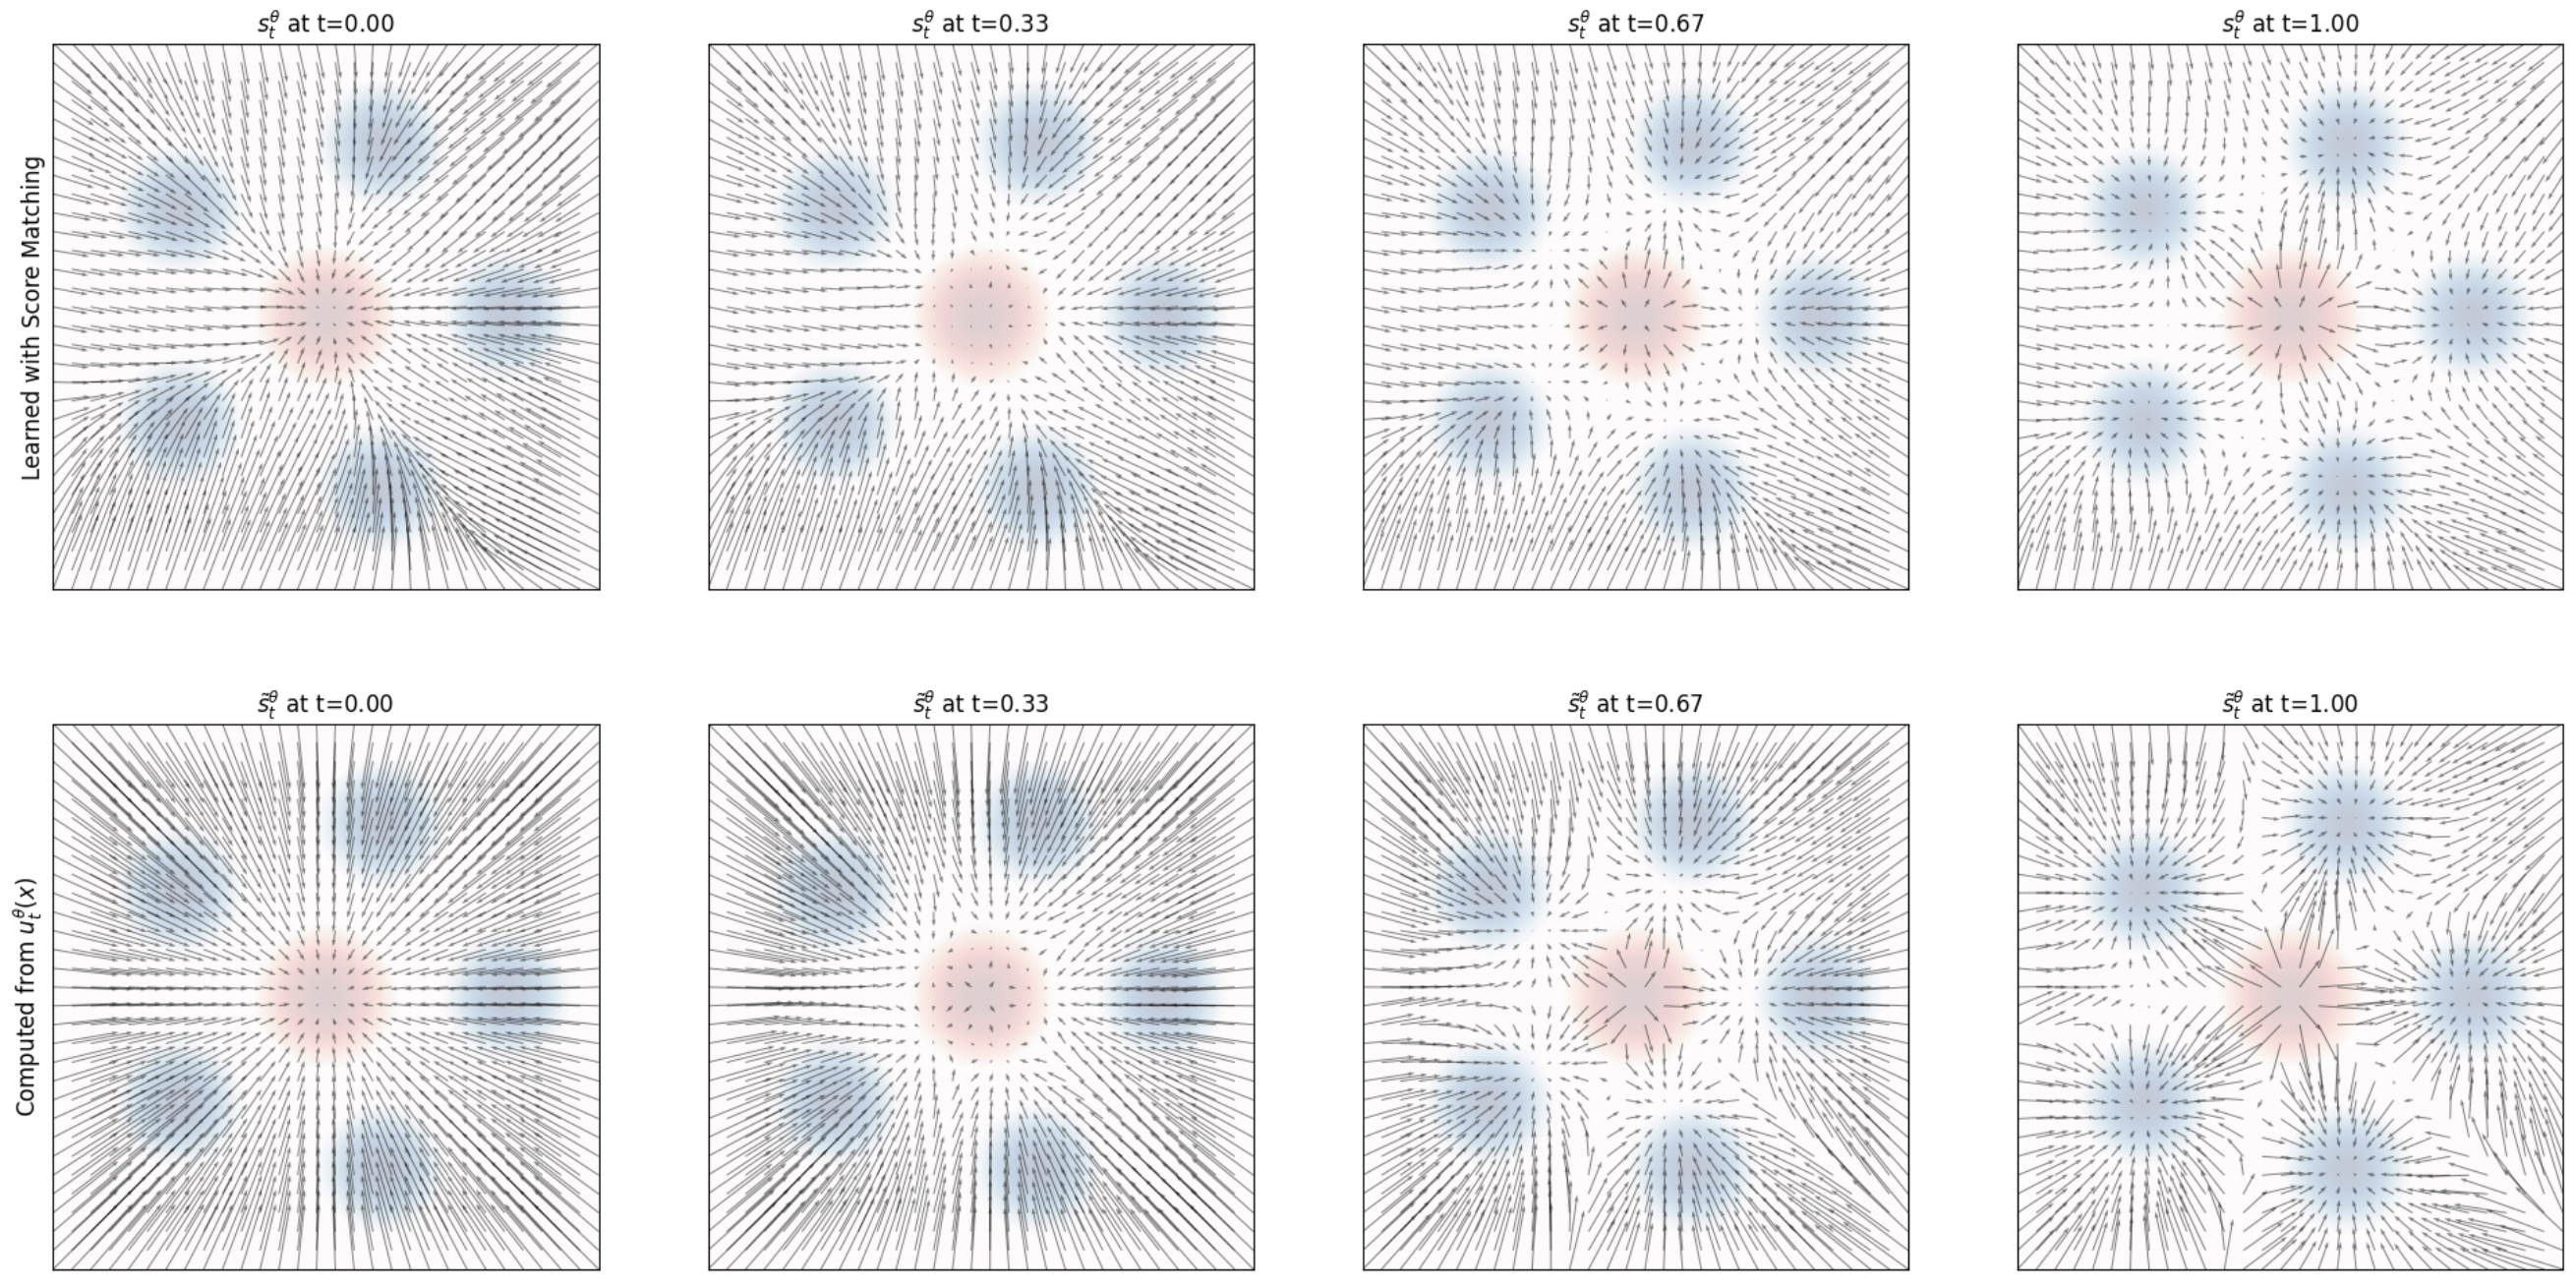
\includegraphics[width=\linewidth]{figures/score_field_comparison.png}
    \caption{\label{fig:score_fields}A comparison of the score, as obtained in two different ways. Top: A visualization of the score field $s_t^\theta(x)$ learned independently with score matching (see \cref{alg:training_score_matching_gaussian_paths}). Bottom: A visualization of the score field $\tilde{s}_t^\theta(x)$ parameterized using $u_t^\theta(x)$ as in \cref{eq:marginal_vf_to_score_formula}.}
\end{figure}
We can use the conversion formula to parameterize the score network $s_t^\theta$ and the vector field network $u_t^\theta$ into one another via 
\begin{align}
u_t^\theta=\left(\beta_t^2\frac{\dot{\alpha}_t}{\alpha_t}-\dot{\beta}_t\beta_t\right)s_t^\theta(x)+\frac{\dot{\alpha}_t}{\alpha_t}x.
\label{eq:marginal_score_to_vf_formula}
\end{align}
Similarly, so long as $\beta_t^2\dot{\alpha}_t -\alpha_t\dot{\beta}_t\beta_t \neq 0$ (always true for $t \in [0,1)$), it follows that
\begin{align}
s_t^\theta(x) = \frac{\alpha_t u_t^\theta(x) - \dot{\alpha}_tx}{\beta_t^2\dot{\alpha}_t -\alpha_t\dot{\beta}_t\beta_t}.
\label{eq:marginal_vf_to_score_formula}
\end{align}
Using this parameterization, it can be shown that the denoising score matching and the conditional flow matching losses are the same up to a constant. We conclude that \textbf{for Gaussian probability paths there is no need to separately train both the marginal score and the marginal vector field, as knowledge of one is sufficient to compute the other. In particular, we can choose whether we want to use flow matching or score matching to train it}. In \cref{fig:score_fields}, we compare visually the score as approximated using score matching and the parameterized score using \cref{eq:marginal_vf_to_score_formula}. If we have trained a score network $s_t^\theta$, we know by \cref{eq:sde_extension_restated} that we can use arbitrary $\sigma_t\geq 0$ to sample from the SDE
\begin{align}
    X_0\sim&\pinit,\quad \dd X_t =\left[\left(\beta_t^2\frac{\dot{\alpha}_t}{\alpha_t}-\dot{\beta}_t\beta_t+\frac{\sigma_t^2}{2}\right)s_t^\theta(x)+\frac{\dot{\alpha}_t}{\alpha_t}x\right]\dd t +\sigma_t\dd W_t
\end{align}
to obtain samples $X_1\sim \pdata$ (up to training and simulation error). This corresponds to \themebf{stochastic sampling from a denoising diffusion model.}


% \subsection{Primer: How to learn conditional expectations}
% We start off by a reminder about some fundamental statistics. Specifically, we briefly discuss on how to approximate (conditional) expectations of some random variables by using the mean squared error.

% \paragraph{Learning an average.} Let us assume that $Z\in\mathbb{R}^k$ is a random variable. Imagine that we want to find the vector $\mathbb{E}[Z]\in\mathbb{R}^k$ given the expected value of $Z$. We can frame this as the following minimization problem of the \themebf{mean squared error}:
% \begin{align}
% \label{eq:average_as_minimization}
%     \mathbb{E}_{Z}[Z] = \argmin\limits_{v\in\mathbb{R}^k}\mathbb{E}_{Z}[\|Z-v\|^2]
% \end{align}
% In other words, the best constant guess $v$ of $Z$ as measured by the mean-squared error is the expected value of $Z$. To see that the above holds, one can do the following calculation for an arbitrary $v$
% \begin{align*}
%     \mathbb{E}[\|Z-v\|^2] =& \mathbb{E}[\|(Z-\mathbb{E}[Z])+(\mathbb{E}[Z]-v)\|^2]\\
% \overset{(i)}{=}&\mathbb{E}[\|Z-\mathbb{E}[Z]\|^2+2(Z-\mathbb{E}[Z])^T(\mathbb{E}[Z]-v)]+\|\mathbb{E}[Z]-v\|^2]\\
% \overset{(ii)}{=}&\mathbb{E}[\|Z-\mathbb{E}[Z]\|^2]+2(\mathbb{E}[Z]-\mathbb{E}[Z])^T(\mathbb{E}[Z]-v)+\|\mathbb{E}[Z]-v\|^2\\
% =&\mathbb{E}[\|Z-\mathbb{E}[Z]\|^2]+\|\mathbb{E}[Z]-v)\|^2\\
% \geq & \mathbb{E}[\|Z-\mathbb{E}[Z]\|^2]
% \end{align*}
% where in $(i)$ we used that identity $\|a+b\|^2=\|a\|^2+2a^Tb+\|b\|^2$ and $(ii)$ we used the fact that the expected value is linear. The last inequality becomes an equality if and only if $v=\mathbb{E}[Z]$. This proves \cref{eq:average_as_minimization}.


% \paragraph{Learning a conditional average.} Let us now imagine that we have two random variables $X\in\mathbb{R}^d,Z\in\mathbb{R}^k$ jointly sampled (i.e. they might be coupled). Let us imagine that we know that $X=x$ and we want to estimate $Z$. Naturally, in machine learning we would choose a parameterized function $F^\theta:\mathbb{R}^d\to\mathbb{R}^k$ (usually $F^\theta$ is a neural network) and then minimize the mean square error
% \begin{align*}
%     L(\theta) =& \mathbb{E}_{X,Z}[\|F^\theta(X)-Z\|^2]
% \end{align*}
% We can 
% \begin{align*}
%     L(\theta) =& \mathbb{E}_{X}[\mathbb{E}[\|F^\theta(X)-Z\|^2|X]]
% \end{align*}
% The best estimate is given by the \themebf{conditional expectation} 
% \begin{align*}
%     F^{\theta^*} = \mathbb{E}[Z|X=x]
% \end{align*}
% Note that the conditional expectation is a function of $x$. How would we approximate it?
% Therefore, we learnt: \textbf{training a neural network by minimizing a mean squared error results in the neural network approximating the conditional expectation.}

%\subsection{Training Algorithm}

\subsection{A Guide to the  Diffusion Model Literature}
\label{subsec:guide_to_flow_matching_literature}

There is a whole family of models around diffusion models and flow matching in the literature. When you read these papers, you will likely find a different (but equivalent) way of presenting the material from this class. This makes it sometimes a little confusing to read these papers. For this reason, we want to give a brief overview over various frameworks and their differences and put them also in their historical context. \textbf{This is not necessary to understand the remainder of this document} but rather intended to be a support for you in case you read the literature.

\paragraph{Discrete time vs. continuous time.} The first denoising diffusion model papers \citep{sohl2015deep, song2019generative, ho2020denoising} did not use SDEs but constructed Markov chains in \themebf{discrete time}, i.e. with time steps $t=0,1,2,3,\dots$. To this date, you will find a lot of works in the literature working with this discrete-time formulation. While this construction is appealing due to its simplicity, the disadvantage of the time-discrete approach is that it forces you to choose a time discretization before training. Further, the loss function needs to be approximated via an \themebf{evidence lower bound (ELBO)} - which is, as the name suggests, only a lower bound to the loss we actually want to minimize. Later, \citet{song2020score} showed that these constructions were essentially an approximation of a time-continuous SDEs. Further, the ELBO loss becomes tight (i.e. it is not a lower bound anymore) in the continuous time case (e.g. note that \cref{thm:fm_loss} and \cref{thm:dsm_loss} are equalities and not lower bounds - this would be different in the discrete time case). This made the SDE construction popular because it was considered mathematically "cleaner" and that one could control the simulation error via ODE/SDE samplers post training. It is important to note however that both models employ the same loss and are \textit{not} fundamentally different.

\paragraph{"Forward process" vs probability paths.} The first wave of denoising diffusion models \citep{sohl2015deep, song2019generative, ho2020denoising, song2020score} did not use the term \themebf{probability path} but constructed a noising procedure of a data point $z\in\mathbb{R}^d$ via a so-called \themebf{forward process}. This is an SDE of the form
\begin{align}
\label{eq:forward_process}
    \bar{X}_0=z,\quad \dd \bar{X}_t = \uforw_t(\bar{X}_t)\dd t + \sigforw_t \dd \bar{W}_t
\end{align}
The idea is that after drawing a data point $z\sim \pdata$ one simulates the forward process and thereby corrupts or "noises" the data. The forward process is designed such that for $t\to \infty$ its distribution converges to a Gaussian $\mathcal{N}(0,I_d)$. In other words, for $T\gg 0$ it holds that $\bar{X}_{T}\sim\mathcal{N}(0,I_d)$ approximately. Note that this essentially corresponds to a probability path: the conditional distribution of $\bar{X}_t$ given $\bar{X}_0=z$ is a conditional probability path $\bar{p}_t(\cdot|z)$ and the distribution of $\bar{X}_t$ marginalized over $z\sim \pdata$ corresponds to a marginal probability path $\bar{p}_t$.\footnote{Note however that they use an \themebf{inverted time convention}: $\bar{p}_0(\cdot|z)=\pdata$ here.} However, note that with this construction, we need to know the distribution of $X_t|X_0=z$ in closed form in order to train our models to avoid simulating the SDE. This essentially restrict the vector field $\uforw_t$ to ones such that we know the distribution $\bar{X}_t|\bar{X}_0=z$ in closed form. Therefore, throughout the diffusion model literature, vector fields in forward processes are always of the affine form, i.e. $\uforw_t(x)=a_t x$ for some continuous function $a_t$. For this choice, we can use known formulas of the conditional distribution \citep{sarkka2019applied,song2021sde, karras2022elucidating}:
\begin{align*}
\bar{X}_t|\bar{X}_0=z\sim\mathcal{N}\left(\alpha_t z,\beta_t^2 I\right),\quad\alpha_t=\exp\parr{\int\limits_{0}^{t}a_r\dd r},\quad\beta_t^2=\alpha_t^2\int\limits_{0}^{t}\frac{(\sigforw_r)^2}{\alpha^2_r}dr
\end{align*}
Note that these are simply Gaussian probability paths. Therefore, one can say that \textbf{a forward process is a specific way of constructing a (Gaussian) probability path.} The term probability path was introduced by flow matching \citep{lipman2022flow} to both simplify the construction and make it more general at the same time: First, the "forward process" of diffusion models is never actually simulated (only samples from $\bar{p}_t(\cdot|z)$ are drawn during training). Second, a forward process only converges for $t\to\infty$ (i.e. we will never arrive at $\pinit$ in finite time). Therefore, we choose to use probability paths in this document.

\paragraph{Time-Reversals vs Solving the Fokker-Planck equation.}

The original description of diffusion models did not construct the training target $\uref_t$ or $\nabla\log p_t$ via the Fokker-Planck equation (or Continuity equation) but via a \themebf{time-reversal} of the forward process \citep{anderson1982reverse}. A time-reversal $(X_t)_{0\leq t\leq T}$ is an SDE with the same distribution over trajectories inverted in time, i.e.
\begin{align}
\mathbb{P}[\bar{X}_{t_1}\in A_1,\dots,\bar{X}_{t_n}\in A_n]=\mathbb{P}[X_{T-t_1}\in A_1,\dots,X_{T-t_n}\in A_n]\\
    \text{ for all }0\leq t_1,\dots, t_n\leq T, \text{ and } A_1,\dots,A_n\subset S
\end{align}
As shown in \citet{anderson1982reverse}, one can obtain a time-reversal satisfying the above condition by the SDE:
\begin{align*}
    \dd X_t =& \left[-u_t(X_t)+\sigma_t^2\nabla\log p_t(X_t)\right]\dd t+ \sigma_{t}\dd W_t,\quad u_t(x)=\uforw_{T-t}(x),\sigma_t=\bar{\sigma}_{T-t}
\end{align*}
As $u_t(X_t)=a_tX_t$, the above corresponds to a specific instance of training target we derived in \cref{prop:conversion_formula_gaussian_prob_path} (this is not immediately trivial as different time conventions are used. See e.g. \citep{lipman2024flow} for a derivation). However, for the purposes of generative modeling, we often only use the final point $X_1$ of the Markov process (e.g., as a generated image) and discard earlier time points. Therefore, whether a Markov process is a ``true'' time-reversal or follows along a probability path does not matter for many applications. Therefore, using a time-reversal is not necessary and often leads to suboptimal results, e.g. the probability flow ODE is often better \citep{karras2022elucidating, ma2024sit}. All ways of sampling from a diffusion models that are different from the time-reversal rely again on using the Fokker-Planck equation. We hope that this illustrates why nowadays many people construct the training targets directly via the Fokker-Planck equation - as pioneered by \citep{lipman2022flow,liu2022flow,albergo2023stochastic} and done in this class.

\paragraph{Flow Matching \citep{lipman2022flow} and Stochastic Interpolants \citep{albergo2023stochastic}.}  The framework that we present is most closely related to the frameworks of flow matching and \themebf{stochastic interpolants (SIs)}. As we learnt, flow matching restricts itself to flows. In fact, one of the key innovations of flow matching was to show that one does not need a construction via a forward process and SDEs but flow models alone can be trained in a scalable manner. Due to this restriction, you should keep in mind that sampling from a flow matching model will be  deterministic (only the initial $X_0\sim \pinit$ will be random). Stochastic interpolants included both the pure flow and the SDE extension via "Langevin dynamics" that we use here (see \cref{thm:langevin_trick}). Stochastic interpolants get their name from a \themebf{interpolant function} $I(t,x,z)$ intended to interpolate between two distributions. In the terminology we use here, this corresponds to a different yet (mainly) equivalent way of constructing a conditional and marginal probability path. The advantage of flow matching and stochastic interpolants over diffusion models is both their simplicity and their generality: their training framework is very simple but at the same time they allow you to go from an arbitrary distribution $\pinit$ to an arbitrary distribution $\pdata$ - while denoising diffusion models only work for Gaussian initial distributions and  Gaussian probability path. This opens up new possibilities for generative modeling that we will touch upon briefly later in this class.

% Denoising diffusion models use a different time convention: First, they use an \themebf{inverted time convention} where time $t=0$ corresponds $\pdata$ and the distribution for $t\to \infty$ is approximately Gaussian. As we have seen in \cref{subsec:diffusion_reference_construction}, diffusion models construct the probability path via a "forward/noising" process and the time-reversal of that process serves as the reference model. As we have seen, this is an equivalent, less general construction. Personally, I found the difference in this convention to flow matching often very confusing. This is unfortunate but very important to keep in mind.

% \paragraph{Stochastic interpolants - \citep{albergo2023stochastic}.} The framework of \themebf{stochastic interpolants (SIs)} is another popular way of constructing generative models via SDEs. It is essentially the framework presented here with a reference SDE constructed via a flow model and a score Langevin model added on top. The name for SI is inspired by the method used in the SI framework to construct probability paths $p_t$. Specifically, the SI framework takes a sample-based perspective, i.e. the marginal probability path $p_t$ is constructed implicitly via a \themebf{interpolant function} $I$. Specifically, let $I:[0,1]\times \mathbb{R}^d\times \mathbb{R}^d\to \mathbb{R}^d$ be a differentiable function such that $I(0,x,z)=x$, $I(1,x,z)=z$ for all $x,z\in \mathbb{R}^d$ and $\gamma:[0,1]\to\mathbb{R}_{>0}$ be such that $\gamma(0)=\gamma(1)=0$. Then define the probability paths implicitly via:
% \begin{align}
% \label{eq:stochastic_interpolant}
% \textbf{Conditional probability path: } &I(t,x,z) + \gamma(t)\epsilon \sim p_t(\cdot|z)\quad (x\sim \pinit, \epsilon\sim \mathcal{N}(0,I_d), \text{ fixed }z)\\
% \textbf{Marginal probability path: }&I(t,x,z) + \gamma(t)\epsilon \sim p_t,\quad (x\sim \pinit, \epsilon\sim \mathcal{N}(0,I_d), z\sim \pdata)
% \end{align}
% By the conditions we imposed on $I,\gamma$, we know that $p_t,p_t(\cdot|z)$ are valid interpolating conditional/marginal probability paths.

Let us summarize the results of this section:
\begin{summarybox}[Training the Generative Model]
\themebf{Flow matching} consists of training a neural network $u_t^\theta$ via minimizing the \themebf{conditional flow matching loss}
\begin{align}
\Lcond(\theta) =     \mathbb{E}_{z\sim \pdata, t\sim \text{Unif},\,x\sim p_t(\cdot|\dap)}[\|u_t^\theta(x) - \uref_t(x|\dap)\|^2]\quad &(\text{conditional flow matching loss})
\end{align}
where $\uref_t(x|z)$ is the conditional vector field (see \cref{alg:training_fm_score_matching_gaussian_paths}). After training, one generates samples by simulating the corresponding ODE (see \cref{alg:sampling_flow_model}). To extend this to a diffusion model, we can use a \themebf{score network} $s_t^\theta$ and train it via \themebf{conditional score matching}
\begin{align}
    \label{eq:dsm}
    \mathcal{L}_{\text{CSM}}(\theta) &= \mathbb{E}_{z\sim \pdata, \,t\sim \text{Unif},\,x\sim p_t(\cdot|\dap)}[\|s_t^\theta(x) - \nabla\log p_t(x|\dap)\|^2] \quad &(\text{denoising score matching loss})
\end{align}
For every diffusion coefficient $\sigma_t\geq 0$, simulating the SDE (e.g. via \cref{alg:sampling_diffusion_model})
\begin{align}
\label{eq:sde_sampling_restated_again}
    X_0\sim&\pinit,\quad \dd X_t =\left[u_t^\theta(X_t)+\frac{\sigma_t^2}{2}s_t^\theta(X_t)\right]\dd t +\sigma_t\dd W_t
\end{align}
will result in generating approximate samples from $\pdata$. One can empirically find the optimal $\sigma_t\geq 0$.\\

\paragraph{Gaussian probability paths.} For the special case of a Gaussian probability path $p_t(x|z)=\mathcal{N}(x;\alpha_tz,\beta_t^2I_d)$, the conditional score matching is also called \themebf{denoising score matching}. This loss and conditional flow matching loss are then given by: 
\begin{align*}
        \mathcal{L}_{\text{CFM}}(\theta) =&\mathbb{E}_{t\sim\Unif,z\sim \pdata, \epsilon\sim \mathcal{N}(0,I_d)}[\|u_t^\theta(\alpha_tz+\beta_t\epsilon)-(\dot{\alpha}_tz+\dot{\beta}_t\epsilon)\|^2]\\
        \mathcal{L}_{\text{CSM}}(\theta)=&\mathbb{E}_{t\sim\Unif,z\sim \pdata, \epsilon\sim \mathcal{N}(0,I_d)}[\|s_t^\theta(\alpha_tz+\beta_t\epsilon)+\frac{\epsilon}{\beta_t}\|^2]
\end{align*}
In this case, there is no need to train $s_t^\theta$ and $u_t^\theta$ separately as we can convert them post training via the formula:
\begin{align*}
u_t^\theta(x)=&\left(\beta_t^2\frac{\dot{\alpha}_t}{\alpha_t}-\dot{\beta}_t\beta_t\right) s_t^\theta(x)+\frac{\dot{\alpha}_t}{\alpha_t}x
\end{align*}
Also here, after training we can simulate the SDE in \cref{eq:sde_sampling_restated_again} via \cref{alg:sampling_diffusion_model} to obtain samples $X_1$.\\

\paragraph{Denoising diffusion models.} 
Denoising diffusion models are diffusion models with Gaussian probability paths. For this reason, it is sufficient for them to learn either $u_t^\theta$ or $s_t^\theta$ as they can be converted into one another. While flow matching only allows for a simulation procedure that is deterministic via ODE, they allow for a simulation that is deterministic (probability flow ODE) or stochastic (SDE sampling). However, unlike flow matching or stochastic interpolants that allow to convert arbitrary distributions $\pinit$ into arbitrary distributions $\pdata$ via arbitrary probability paths $p_t$, denoising diffusion models only works for Gaussian initial distributions $\pinit=\mathcal{N}(0,I_d)$ and a Gaussian probability path.\\

\paragraph{Literature} Alternative formulations for diffusion models that are popular in the literature are:
\begin{enumerate}
    \item \textbf{\sffamily Discrete-time: }Approximations of SDEs via discrete-time Markov chains are often used.
    \item \textbf{\sffamily Inverted time convention: }It is popular to use an inverted time convention where $t=0$ corresponds to $\pdata$ (as opposed to here where $t=0$ corresponds to $\pinit$).
    \item \textbf{\sffamily Forward process: }Forward processes (or noising processes) are ways of constructing (Gaussian) probability paths.
    \item \textbf{\sffamily Training target via time-reversal:} A training target can also be  constructed via the time-reversal of SDEs. This is a specific instance of the construction presented here (with an inverted time convention).
\end{enumerate}
\end{summarybox}
% \paragraph{Adding noise to data.}

% \paragraph{Frame as probability path.}

% \paragraph{How do I go the other way?} Transport mass - using Fokker-Planck equation.

% \paragraph{Weak time-reversal.} Probability flow ODE.

% \paragraph{Adding Langevin dynamics.}

% \paragraph{Special case: Proper time-reversal.}

% \paragraph{Specify marginals via an SDE.} Example of Ohrnstein-Uhlenbeck process.

% Instantaneous Change of Variables (evaluating log-likelihood).
% Deterministic sampling. Stochastic sampling:
% Linear ODEs, SDEs with affine drift coefficients, Time-reversal idea.